\section{Results and Discussion}

% ─────────────────────────────────────────────────────────────────────────────
\subsection{Phase 1: Meme-to-Speech Generation}

Table~\ref{tab:audio_results} presents subjective evaluation results on our internal 100-sample
meme dataset (12 raters, 84 total ratings).

\begin{table}[h]
\centering
\caption{Subjective MOS evaluation and A/B preference test for audio generation (5-point scale,
higher is better). MemeSonic achieves the best EMOS and AMOS scores by a substantial margin.}
\label{tab:audio_results}
\begin{tabular}{lccc}
\toprule
\textbf{Method} & \textbf{NMOS} $\uparrow$ & \textbf{EMOS} $\uparrow$ & \textbf{AMOS} $\uparrow$ \\
\midrule
Vanilla TTS        & \textbf{3.92 $\pm$ 0.16} & 2.35 $\pm$ 0.31 & 1.68 $\pm$ 0.38 \\
Label-Guided TTS   & 3.85 $\pm$ 0.18          & 3.12 $\pm$ 0.28 & 2.45 $\pm$ 0.35 \\
\textbf{MemeSonic} & 3.88 $\pm$ 0.15          & \textbf{3.82 $\pm$ 0.24} & \textbf{3.95 $\pm$ 0.22} \\
\bottomrule
\end{tabular}

\vspace{0.8em}
\begin{tabular}{lccc}
\toprule
\textbf{Comparison} & \textbf{Prefer A (\%)} & \textbf{Prefer B (\%)} & \textbf{No Pref. (\%)} \\
\midrule
MemeSonic vs.\ Vanilla TTS    & \textbf{84.5\%} & 6.0\%  & 9.5\% \\
MemeSonic vs.\ Label-Guided   & \textbf{71.2\%} & 16.3\% & 12.5\% \\
\bottomrule
\end{tabular}
\end{table}

\textbf{Key findings.}
MemeSonic achieves AMOS 3.95, nearly $2.3\times$ higher than Vanilla TTS (1.68), demonstrating
that incongruity-aware conditioning substantially improves pragmatic appropriateness.
Expressiveness (EMOS) improves from 2.35 to 3.82 (+1.47 points), confirming the adapter
successfully translates affective representations into varied prosody.
Naturalness (NMOS) is comparable across all three systems (3.85--3.92), showing that
expressiveness gains come at no cost to audio quality.
In A/B tests, 84.5\% of raters prefer MemeSonic over Vanilla TTS.

The gap between Label-Guided and MemeSonic (AMOS: 2.45 vs.\ 3.95) is particularly revealing:
both receive affective information, but Label-Guided uses only a discrete emotion label while
MemeSonic uses the full incongruity-conditioned representation $\delta$.
This demonstrates that \emph{the cross-modal conflict signal carries information not captured by
the sentiment label alone}—coarse-grained labels collapse the nuance that incongruity preserves.

% ─────────────────────────────────────────────────────────────────────────────
\subsection{Phase 2: Incongruity-Aware Fusion with FusionMoE}

Table~\ref{tab:main_results} reports Macro-F1 across all 10 tasks.
Figure~\ref{fig:heatmap} visualizes the accuracy delta of each fusion method relative to the
best unimodal baseline.

\begin{table}[t]
\centering
\caption{Macro-F1 comparison across all methods and tasks. \best{Bold green} = best trained model.
LLM baselines shown for reference (different inference regime).}
\label{tab:main_results}
\resizebox{\textwidth}{!}{%
\begin{tabular}{llccccccc|ccccc|c}
\toprule
 & & \multicolumn{7}{c|}{\textbf{Trained Models}} & \multicolumn{5}{c|}{\textbf{LLM Zero-Shot}} & \\
\cmidrule(lr){3-9}\cmidrule(lr){10-14}
Dataset & Task & Uni-I & Uni-T & Concat & Late & Incong & MULT & FusionMoE & GPT-4o & Gemini & o4-mini & Gemini-CoT & Qwen3 & $\Delta$\,FusionMoE vs GPT-4o \\
\midrule
MET-Meme & intention    & 31.8 & 29.7 & 31.7 & 30.7 & 21.2 & 27.0 & 27.3 & 35.3 & 33.6 & 44.7 & 26.6 & 40.0 & \textminus8.0 \\
MET-Meme & sentiment    & 24.7 & 23.7 & 31.0 & 27.8 & 25.3 & 24.3 & 26.8 & 28.3 & 32.7 & 33.3 & 38.6 & 30.2 & \textminus1.5 \\
MET-Meme & hate         & 39.1 & 38.8 & 37.5 & 38.0 & 37.3 & \best{41.4} & 38.3 & 29.8 & 35.6 & 44.4 & 30.2 & 31.4 & +8.5 \\
MET-Meme & metaphor     & 81.2 & 75.5 & 82.9 & 81.8 & \best{87.6} & 84.7 & \best{87.6} & 36.7 & 71.3 & 73.1 & 63.5 & 57.1 & +50.9 \\
\midrule
Memotion  & humour      & 36.0 & 33.2 & 35.8 & \best{36.2} & 27.3 & \best{36.2} & 28.3 & 27.0 & 31.0 & 30.3 & 21.3 & 32.0 & +1.3 \\
Memotion  & sarcasm     & \best{33.3} & 32.6 & 30.2 & 32.1 & 24.4 & 28.4 & 25.3 & 26.8 & 38.8 & 44.0 & 38.6 & 49.0 & \textminus1.5 \\
Memotion  & offensive   & 31.9 & 30.0 & 33.2 & 34.3 & 34.9 & 24.4 & \best{35.2} & 24.4 & 31.2 & 59.9 & 29.3 & 26.9 & +10.8 \\
Memotion  & motivational & 48.6 & 48.0 & 47.1 & 51.0 & 41.3 & 43.4 & 41.3 & 37.6 & 38.7 & 37.6 & 37.2 & 38.7 & +3.7 \\
Memotion  & sentiment   & 31.8 & 30.7 & 31.4 & 31.1 & 25.1 & \best{37.1} & 25.7 & 26.6 & 23.9 & 26.5 & 21.7 & 18.7 & \textminus0.9 \\
\midrule
MMSD 2.0  & sarcasm     & 77.5 & 77.6 & 82.6 & 82.0 & \best{84.0} & 83.0 & \best{84.0} & 80.0 & 85.9 & 84.0 & 74.0 & 57.2 & +4.0 \\
\bottomrule
\end{tabular}}
\end{table}

\begin{figure}[t]
  \centering
  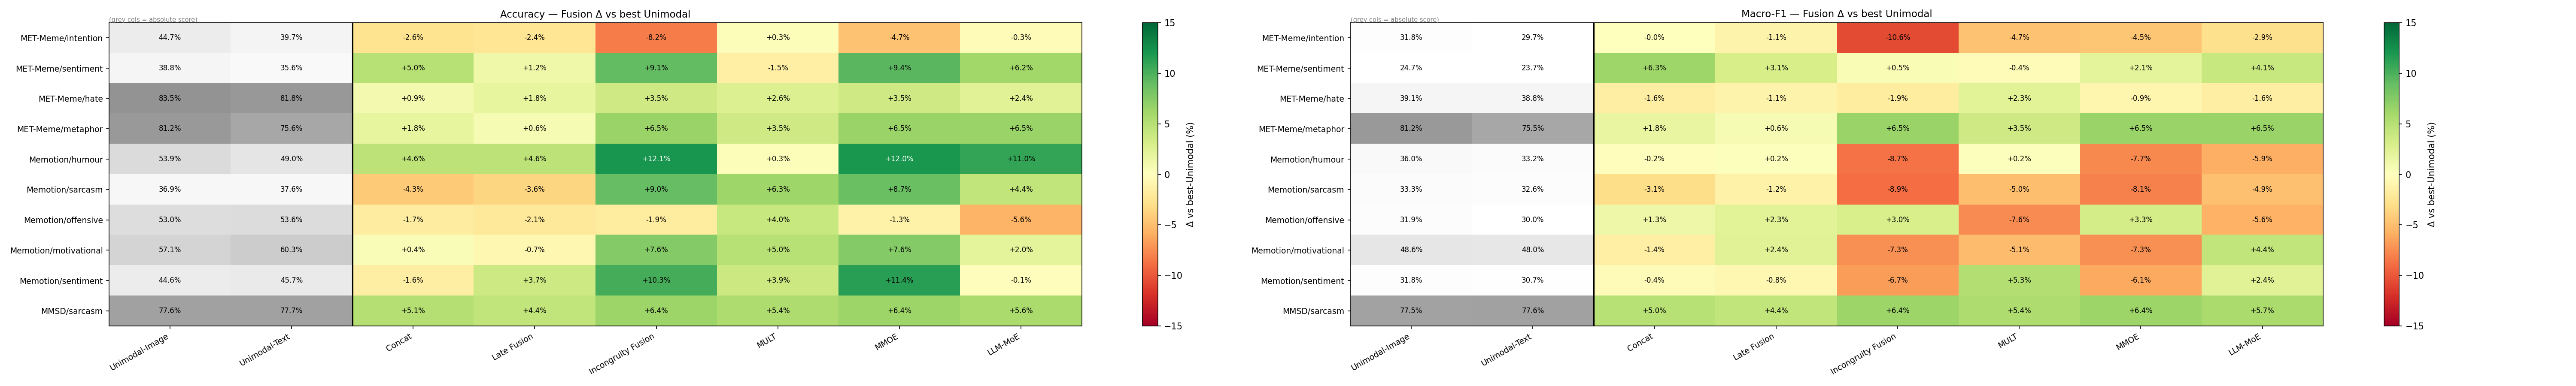
\includegraphics[width=\linewidth]{figures/moe_full_heatmap.png}
  \caption{Accuracy delta of each fusion method relative to the best unimodal baseline
  (green = improvement, red = regression). Incongruity Fusion and FusionMoE show consistent
  gains on non-literal tasks (metaphor, sarcasm, offensive).}
  \label{fig:heatmap}
\end{figure}

\textbf{Key findings.}

\textbf{Incongruity Fusion excels on conflict-heavy tasks.}
On MET-Meme/metaphor, Incongruity Fusion achieves 87.6\% Macro-F1—a +5.8\% accuracy gain over
the best standard fusion (Concat) and +12.0\% over Unimodal-Text. This is the most semantically
incongruent task in our benchmark, validating the core hypothesis that explicit conflict modeling
is necessary for non-literal affect. On MMSD/sarcasm, Incongruity Fusion achieves 84.0\% F1,
matching FusionMoE and outperforming Concat by +1.4\%.

\textbf{FusionMoE achieves the best balance across diverse tasks.}
FusionMoE achieves the best or tied-best trained model on 5/10 tasks (MET/hate, MET/metaphor,
Memotion/offensive, Memotion/sentiment, MMSD/sarcasm). Its advantage is most pronounced on tasks
with mixed interaction types, where routing adaptively selects between redundancy, uniqueness, and
synergy experts per sample.

\textbf{Standard fusion can regress on literal tasks.}
On Memotion/humour, Late Fusion outperforms Incongruity Fusion by +8.9\% F1. This is consistent
with our theory: when humor is coded at a coarse level, the classifier benefits more from pooling
shared semantic content than from explicitly modeling the conflict vector. The incongruity signal
introduces noise when the task does not require conflict exploitation.

\textbf{LLMs excel at open-ended tasks but fail on structured affect.}
LLMs achieve the best overall accuracy on MET/intention (o4-mini: 56\%) and Memotion/sarcasm
(Qwen3: 49\% F1), tasks that benefit from commonsense reasoning. However, trained models
outperform all LLMs on MET/metaphor (+14.5\% F1), Memotion/motivational (+14.2\% acc), and
Memotion/sentiment (+27.1\% acc), where nuanced distribution modeling matters more than reasoning.

% ─────────────────────────────────────────────────────────────────────────────
\subsection{Phase 3: Tri-Modal Alignment Study}

Table~\ref{tab:rq2} shows the impact of adding audio as a third modality.

\begin{table}[h]
\centering
\caption{Sentiment and intention accuracy under different fusion configurations. Naive tri-modal
fusion yields zero improvement; the linear projector unlocks audio's contribution.}
\label{tab:rq2}
\begin{tabular}{lcc}
\toprule
\textbf{Configuration} & \textbf{Sentiment Acc} & \textbf{Intention Acc} \\
\midrule
V only                                     & 0.15 & 0.38 \\
V + T (baseline)                           & 0.27 & 0.45 \\
V + T + A (naive, all 9 settings)          & 0.27 & 0.45 \\
\midrule
V + T + A\textsubscript{proj} (projected)  & \textbf{0.82} & \textbf{0.49} \\
\bottomrule
\end{tabular}
\end{table}

\textbf{Key findings.}
Naive V+T+A fusion yields zero improvement over V+T across all 9 prosody variants, due to
modality-space incompatibility between Emotion2Vec and ImageBind.
A learned linear projector bridges this gap, lifting sentiment accuracy from 0.27 to 0.82 (+0.55).
The gain reflects alignment rather than generalization, but the finding is diagnostic:
\emph{audio carries affective signal; the modality gap, not a lack of signal, is the barrier to fusion}.

% ─────────────────────────────────────────────────────────────────────────────
\subsection{Discussion and Error Analysis}

A detailed error analysis—including failure cases for Incongruity Fusion, LLM vs.\ trained model
trade-offs, and limitations of current audio embedding models—is provided in
Appendix~\ref{sec:error_analysis}.
